%!TEX root = ../../../thesis.tex

\section{Operational Model}

In this section we will develop a model of operation for a streaming cell.
This helps to determine what parameters are important when maximising the output power of a cell.

\subsection{Mathematics of streaming}

Before building and measuring any streaming cells, lets look briefly at the mathematics governing them.
Rigorous mathematical analysis of streaming cell performance is extremely involved and is will detailed in the literature \cite{Yang1998}.
It is still a matter of debate as the structure of the double layer itself is still not fully understood.

\subsubsection*{Streaming voltages}

In \cite{Gu2000a}, the ratio of streaming voltage to applied pressure is derived for a rectangular, parallel plate micro-channel.
This is shown in \cref{eq:streamingVoltage_with_pressure}.

\begin{equation}
\frac{V_{s}}{\Delta P_{z}} = \frac{\varepsilon_{0}\,\varepsilon_{0}\,\zeta}{\mu[\lambda_{b}+2(\frac{1}{W}-\frac{1}{\delta})\lambda_{S}]}
\label{eq:streamingVoltage_with_pressure}
\end{equation}

\noindent where:
\begin{description}
    \item $V_{s}$ is the streaming voltage
    \item $\Delta P_{z}$ is the pressure differential across the channel
    \item $\epsilon_{r}$ is the relative permittivity of the liquid
    \item $\epsilon_{0}$ is the absolute permittivity of free space
    \item $\zeta$ is the zeta potential of the solid-liquid interface
    \item $\lambda_{b}$ is the bulk conductivity of the liquid
    \item $W$ is the width of the channel
    \item $\delta$ is the height of the channel
    \item $\lambda_{s}$ is the surface conductivity of the channel
\end{description}

This equation is important as it is specific to the type of channels fabricated in this work.
Later, we will measure the streaming voltage to applied pressure ratio.
This equation allows for us to determine both the surface conductivity of the channel and its zeta potential.

\subsubsection*{Streaming current}

A much more crude mathematical model representing the steaming current in a porous plug is given by Olthuis et. al in \cite{Olthuis2005}, and is shown here as \ref{eq:StreamingCell_StreamingCurrentFunc}

\begin{equation}
    I_{s}=\frac{A\,\varepsilon_{0\,}\varepsilon_{r}}{\eta\,l}\Delta P\,\zeta
    \label{eq:StreamingCell_StreamingCurrentFunc}
\end{equation}
where:

\begin{description}
    \item [{$A$}] is the cross-sectional area of the channel
    \item [{$\varepsilon_{0}$}] is the permittivity of free space
    \item [{$\varepsilon_{r}$}] is the relative permittivity of the liquid
    \item [{$\eta$}] is the viscosity of the liquid
    \item [{$l$}] is the length of the channel
    \item [{$\Delta P$}] is the pressure difference across the channel
    \item [{$\zeta$}] is the zeta-potential of the solid-liquid interface
\end{description}
This equation indicates that the cell will produce a current that is proportional to the amount of pressure across it and
that the output is affected by the geometry of the channel itself.


To help model the situation it is convenient to break \cref{eq:StreamingCell_StreamingCurrentFunc} down in the following
manner:

\pagebreak
\begin{align}
    I_{s} & = \Delta P\,\left(\frac{A}{\eta\,l}\right)\,\left(\varepsilon_{0}\,\varepsilon_{r}\,\zeta\right)\nonumber\\
    \label{eq:streaming_current_rearranged}I_{s} & = \frac{\Delta P}{\left(\frac{\eta\,l}{A}\right)}\,\left(\varepsilon_{0}\,\varepsilon_{r}\,\zeta\right)
\end{align}

This is a useful step since $\frac{\eta\,l}{A}$ is equivalent to the hydrostatic resistance of the channel.
Knowing this, we can substitute this hydrostatic resistance into \cref{eq:streaming_current_rearranged} as $R_{h}$, yielding

\begin{align}
    I_{s} & = \frac{\Delta P}{R_{h}}\,\left(\varepsilon_{0}\,\varepsilon_{r}\,\zeta\right)\nonumber\\
    \frac{I_{s}}{\Delta P} & =\frac{\varepsilon_{0}\,\varepsilon_{r}\,\zeta}{R_{h}}\nonumber \\
    g_{m} & = \frac{\varepsilon_{0}\,\varepsilon_{r}\,\zeta}{R_{h}}
\end{align}

where $R_{h}$ is the hydrodynamic resistance caused by the channel, $g_{m}$ represents the transconductance between pressure applied and current produced and $I_{s}$ is the streaming current.
The hydrodynamic resistance ($R_{h}$) will be affected by the geometry of the channel so $R_{h}$ is considered an approximation of the hydrodynamic resistance.

Once the cell begins to separate charge, a current in the reverse direction is established called the conduction current ($I_{c}$).

As Ohm's law states:

\[ I=\frac{V}{R} \]

In this situation the resistance is determined by the conductivity of the water
($\sigma$), as well as the cross sectional area ($A$) and length ($l$) of the
channel.

\[ R=\frac{l}{\sigma\, A} \]


Therefore, the conduction current back through the channel is determined by:

\begin{equation} I_{c}=A\sigma\frac{V_{s}}{l} \end{equation}


Where $\sigma$ is the conductivity of the liquid and $V_{s}$ is the voltage
developed across the channel.

At equilibrium the streaming current ($I_{s}$) and the conduction current
($I_{c}$) are equal and opposite in direction.


\subsection{\label{sub:Electrical-model}Electrical model}

Figure \ref{fig:StreamingCell_Schematic-representation} depicts schematically how a streaming cell would operate when connected to an external load.
This model is based upon that found in \cite{Olthuis2005}, but has been modified to show the product of pressure applied ($\Delta P$) and the zeta potential ($\zeta$) as the voltage source.
This is opposed to \cite{Olthuis2005}, who show solely the zeta potential as the input parameter.
It is the pressure differential across the cell that transports the charge available; a zeta potential on its own simply isn't enough.
This has been shown through the results obtained in Appendix \ref{sec:Appendix-Streaming-Potential-Cell}, where $V_{s}$ was directly proportional to $\Delta P$; as $V_{s}$ is directly related to $I_{s}$ as per Ohm's law.

\begin{figure}
    \centering
        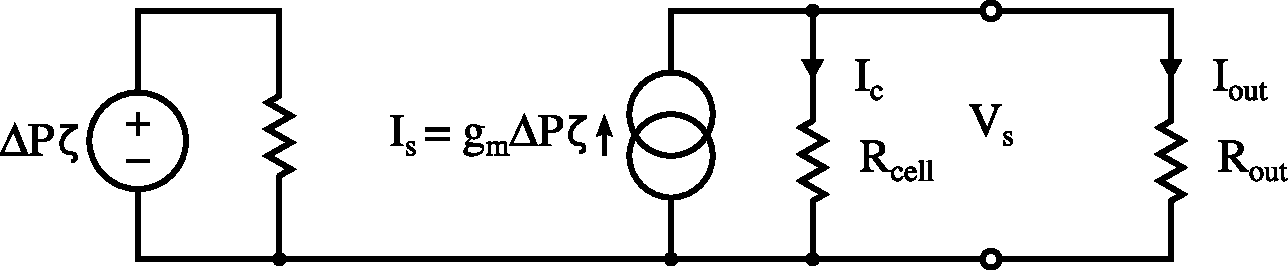
\includegraphics[width=\textwidth]{content/pt1/01-PowerHarvesting/graphics/StreamingCell_EquivalentCircuit_output}
    \caption{\label{fig:StreamingCell_Schematic-representation}Schematic representation of a streaming cell with attached output resistance}
\end{figure}



\subsection{Output analysis}

The model described in \ref{sub:Electrical-model} depicts how the cell would operate with a load resistance placed across its ends ($R_{out}$).
From this model we can see that putting a load across the cell actually places it in parallel with the cells own internal electrical resistance ($R_{cell}$).
The most important aspect of the cell is its output power.
How does choosing the value of load resistance ($R_{out}$) affect the output power?


\subsubsection*{Finding an optimum value for $R_{out}$}

Using Ohm's Law it is possible to form an equation linking the total power ($P_{cell}$) to the total electrical resistance across the cell ($R_{tot}$).

\begin{eqnarray}
    P & = & V\times I\nonumber \\
    V & = & I\times R\nonumber \\
    P & = & I^{2}\times R\nonumber \\
    P_{cell} & = & I_{s}^{2}\times R_{tot}
    \label{eq:DeterminingOutputPower_basic}
\end{eqnarray}

Where $I_{s}$ is the streaming current created by pumping ions through the channel.
As the output resistance and internal cell resistance are in parallel we can find the output current ($I_{out}$) by treating the cell as a resistor divider.

\begin{eqnarray}
    I_{out} & = & I_{s}\times\frac{R_{cell}}{R_{cell}+R_{out}}
    \label{eq:DeterminingOutputPower_extended}
\end{eqnarray}

Combining \eqref{eq:DeterminingOutputPower_basic} and \eqref{eq:DeterminingOutputPower_extended} we can extract the power dissipated in a load attached across the cell.

\begin{eqnarray}
    I_{out} & = & I_{s}\times\frac{R_{cell}}{R_{cell}+R_{out}}\nonumber \\
    P_{out} & = & \left[I_{s}\times\frac{R_{cell}}{R_{cell}+R_{out}}\right]^{2}\times R_{out}
    \label{eq:DeterminingOutputPower_result}
\end{eqnarray}

Equation \eqref{eq:DeterminingOutputPower_result} takes into account the internal dissipation within the cell due to its own internal resistance.
In order to optimise the output power it is necessary to find the value of output resistance ($R_{out}$) that maximises the output power.

A parallel resistance system where we try to maximise the output power suggests this is a maximum power transfer theorem problem.
The maximum power transfer theorem states that in order to maximise the power delivered to an external load from a source which itself has an internal resistance, one must make the two resistance equal.

\subsubsection*{Maximum power transfer theorem for a current source}
This theorem is shown for resistors in series but no clear proof was found for a current source with two resistances in parallel.
Here I prove that the maximum power theorem holds for a current source with resistors in parallel.

First I take Equation \ref{eq:DeterminingOutputPower_result} and treat the streaming current ($I_{s}$) as a constant, differentiate with respect to $R_{out}$ and find the condition that gives a maximum/minimum power output.

\begin{eqnarray}
    P_{out} & = & \left[I_{s}\times\frac{R_{cell}}{R_{cell}+R_{out}}\right]^{2}\times R_{out}\nonumber\\
    \frac{P_{out}}{R_{out}} & = & \left[1\times\frac{R_{cell}}{R_{cell}+R_{out}}\right]^{2}\nonumber\\
    \frac{\partial P_{out}}{\partial R_{out}} & = & \frac{R_{cell}^{2}}{(R_{cell}+R_{out})^{2}}-\frac{2\times R_{cell}^{2}\times R_{out}}{(R_{cell}+R_{out})^{3}}\nonumber\\
    0 & = & \frac{R_{cell}^{2}}{(R_{cell}+R_{out})^{2}}-\frac{2\times R_{cell}^{2}\times R_{out}}{(R_{cell}+R_{out})^{3}}\nonumber\\
    \frac{2\times R_{cell}^{2}\times R_{out}}{(R_{cell}+R_{out})^{3}} & = & \frac{R_{cell}^{2}}{(R_{cell}+R_{out})^{2}}\nonumber\\
    \frac{2\times R_{cell}^{2}\times R_{out}}{R_{cell}+R_{out}} & = & R_{cell}^{2}\nonumber\\
    2\times R_{cell}^{2}\times R_{out} & = & R_{cell}^{2}\times(R_{cell}+R_{out})\nonumber\\
    2\times R_{out} & = & R_{cell}+R_{out}\nonumber\\
    R_{out} & = & R_{cell}
    \label{eq:maximumPowerTheorem_norton}
\end{eqnarray}

This shows that there is either maximum or minimum power transfer to $R_{out}$ when the value of $R_{out}$ matches that of $R_{cell}$.
By plotting the power output as a function of the ratio of the two resistances (shown in \cref{fig:Plot-of-PowerTheorem}), we can see it is indeed a maximum.
This shows the assumption of the maximum power transfer theorem in the case of streaming cell output to be correct.
Usefully, it is shown that the absolute magnitudes of both $R_{out}$ and $R_{cell}$ have no effect on the output power.

\begin{figure}
    \centering
        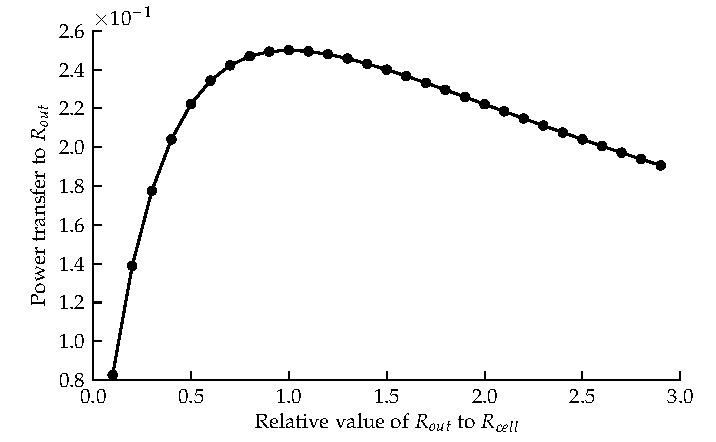
\includegraphics{content/pt1/01-PowerHarvesting/graphics/maximumPowerThereom}
    \caption{\label{fig:Plot-of-PowerTheorem}Plot of Equation \ref{eq:DeterminingOutputPower_result} when $I_{s}=1A$ and $R_{cell}=1\Omega$}
\end{figure}

\subsubsection*{Optimising streaming cell parameters}

This can now be used to calculate the maximum available power as a function of
$I_{s}$ by substituting $R_{out}$ and $R_{cell}$ for $R$ , as
$R_{out}=R_{cell}=R$:

\begin{eqnarray} P_{out} & = &
    \left[I_{s}\times\frac{R_{cell}}{R_{cell}+R_{out}}\right]^{2}\times
    R_{out}\nonumber \\ P_{max} & = &
    \left[I_{s}\times\frac{1}{2}\right]^{2}\times R\nonumber \\ P_{max} & = &
    \frac{I_{s}^{2}R}{2}\label{eq:streamingCell_maxPower} \end{eqnarray}


And as $P=I^{2}R$ (via the power equation and Ohm's Law) this indicates that at
most we can hope to havest half of the total power, while the other half is
dissipated back through $R_{cell}$. Combining Equations
\ref{eq:streamingCell_maxPower} and
\ref{eq:StreamingCurrent_HydrostaticResistance} gives:

\begin{eqnarray*} P_{max} & = & \frac{\left(\frac{\Delta
                P}{R_{h}}\,\left(\varepsilon_{0}\,\varepsilon_{r}\,\zeta\right)\right)^{2}R}{2}\\
    P_{max} & = & \frac{\left(\frac{\Delta
                P\,\varepsilon\,\zeta}{R_{h}}\right)^{2}R}{2}\\ P_{max} & = &
    \frac{\Delta P^{2}\,\varepsilon^{2}\,\zeta^{2}R}{2R_{h}^{2}}
\end{eqnarray*}


where $\varepsilon=\varepsilon_{0}\,\varepsilon_{r}$ and $R=R_{cell}=R_{out}$ .
If we now substitute $R$ and $R_{h}$ for their respective functions we end up
with:

\begin{eqnarray} P_{max} & = & \frac{\Delta
        P^{2}\,\varepsilon^{2}\,\zeta^{2}R}{2R_{h}^{2}}\nonumber \\ P_{max} & =
    & \frac{\Delta P^{2}\,\varepsilon^{2}\,\zeta^{2}\,\left(\frac{l}{\sigma\,
                A}\right)}{2\left(\frac{\eta\, l}{A}\right)_{h}^{2}}\nonumber
    \\ P_{max} & = & \frac{\Delta P^{2}\,\varepsilon^{2}\,\zeta^{2}\,
        l}{\sigma\, A}\times\frac{1}{\frac{2\eta^{2}\, l^{2}}{A^{2}}}\nonumber
    \\ P_{max} & = & \frac{\Delta P^{2}\,\varepsilon^{2}\,\zeta^{2}\, l\,
        A^{2}}{\sigma\, A\,2\eta^{2}\, l^{2}}\nonumber \\ P_{max} & = &
    \frac{\Delta P^{2}\,\varepsilon^{2}\,\zeta^{2}\, A}{2\,\sigma\,\eta^{2}\,
        l}\nonumber \\ P_{max} & \propto & \frac{\Delta P^{2}\,\zeta^{2}\,
        A}{l}\nonumber \\ P_{max} & \propto & \frac{\Delta
        P^{2}\,\zeta^{2}}{R_{h}} \end{eqnarray}



\subsubsection*{Optimisation of $R_{h}$ and $\Delta P$}

Knowing the optimum value of output resitance leaves only the streaming current
($I_{s}$) and it's constituants as optimisation parameters.  Equation
\ref{eq:StreamingCurrent_HydrostaticResistance} indicates that in order to
further optimise the cell, one must reduce hydrodynamic resistance ($R_{h}$)
and increase both the Zeta potential ($\xi$) and pressure difference ($\Delta
P$) placed across the cell.

We can model the water supply, harvester and a consumer as a basic electrical
circuit as shown in Figure \ref{fig:Schematic-model-of-harvester}.  In this
model $P_{supply}$ represents the total water pressure available, Flow
represents the flow rate of water, $R_{h}$ and $R_{consumer}$ are the
hydrodynamic resistances of the harvesting cell and a water consumer (e.g. a
house) respecively and $\Delta P$ is the pressure developed difference across
the harvester, where $R_{h}\propto\frac{l}{A}$.

\begin{figure} \begin{centering}
        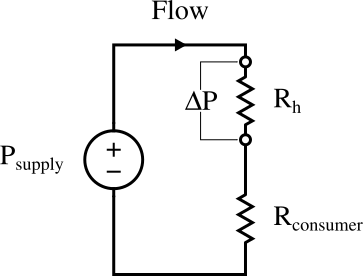
\includegraphics[scale=0.55]{content/pt1/01-PowerHarvesting/graphics/Harvester_equivalentCircuit_output}
        \par\end{centering}

\protect\caption{\label{fig:Schematic-model-of-harvester}Schematic model of the
    water supply, harvester and consumer}


\end{figure}


\begin{figure} \begin{centering}
        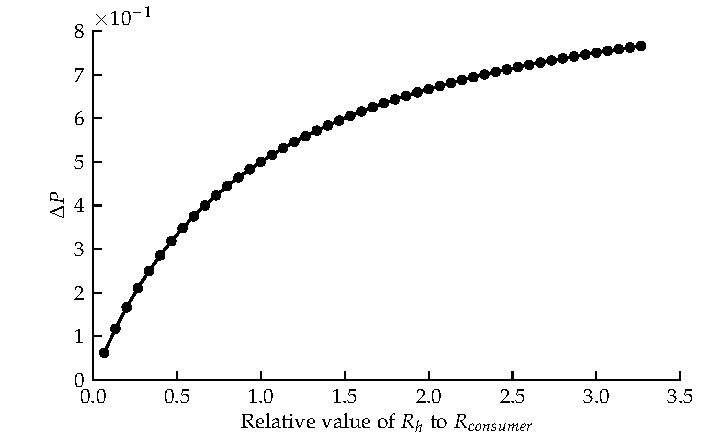
\includegraphics{content/pt1/01-PowerHarvesting/graphics/streamingCell_consumerModel_dP}
        \par\end{centering}

\protect\caption{\label{fig:Effect-of-varying-Rh-onP}Effect of varying $R_{h}$
    on $\Delta P$ for the harvester/consumer model shown in Figure
    \ref{fig:Schematic-model-of-harvester}.}


\end{figure}


\begin{figure} \begin{centering}
        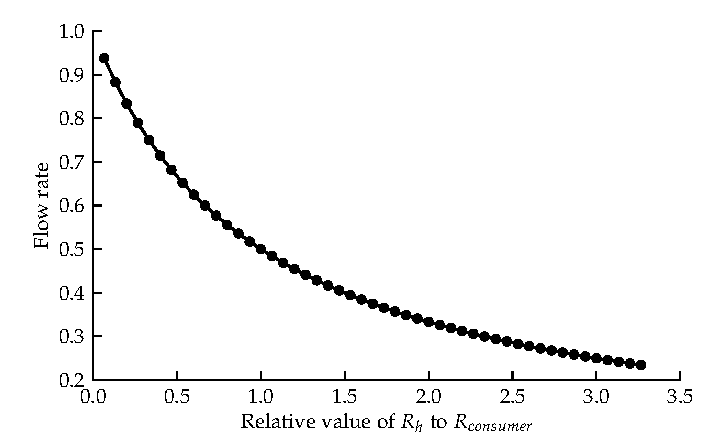
\includegraphics{content/pt1/01-PowerHarvesting/graphics/streamingCell_consumerModel_flow}
        \par\end{centering}

\protect\caption{\label{fig:Effect-of-varying-Rh-onFlow}Effect of varying
    $R_{h}$ on Flow for the harvester/consumer model shown in Figure
    \ref{fig:Schematic-model-of-harvester}.} \end{figure}


\begin{figure} \begin{centering}
        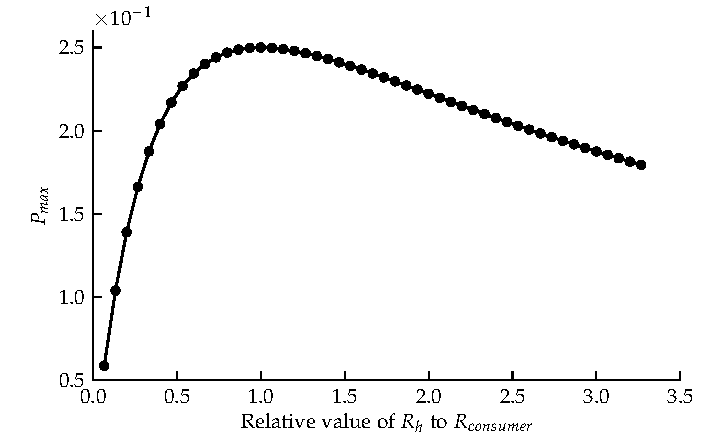
\includegraphics{content/pt1/01-PowerHarvesting/graphics/streamingCell_consumerModel_total}
        \par\end{centering}

\protect\caption{\label{fig:Effect-of-varying-Rh-onIs}Effect of varying $R_{h}$
    on \foreignlanguage{english}{$P_{max}$} for the harvester/consumer model
    shown in Figure \ref{fig:Schematic-model-of-harvester}.} \end{figure}
Figures \ref{fig:Effect-of-varying-Rh-onP},
\ref{fig:Effect-of-varying-Rh-onFlow} and \ref{fig:Effect-of-varying-Rh-onIs}
show how varying $R_{h}$ will affect $\Delta P$, the flow rate and the value of
$\frac{\Delta P}{R_{h}}$ respectively. Notice in Figure
\ref{fig:Effect-of-varying-Rh-onP} that increasing $R_{h}$ has the effect of
increasing $\Delta P$.  Optimisation wise, the benifit of increasing $I_{s}$ by
increasing $\Delta P$ is opposed by also increasing the value of $R_{h}$
(referring to Equation \ref{eq:StreamingCurrent_HydrostaticResistance}).

Figure \ref{fig:Effect-of-varying-Rh-onFlow} shows how the value of $R_{h}$
affects the flow rate through the system. Keeping the flow rate high is
important in order to ensure that the consumer does not notice a drop in water
pressure due to the addition of the harvester in their water system.

Finally, Figure \ref{fig:Effect-of-varying-Rh-onIs} shows the effect that
varying $R_{h}$ has on \foreignlanguage{english}{$P_{max}$} (according to
$P_{max}\propto\frac{\Delta P^{2}\,\zeta^{2}}{R_{h}}$ when $\zeta=1$). The
result is the same as that of Equation \ref{eq:DeterminingOutputPower}, showing
that this is again goverend by the maximum power transfer thereom. Practically,
a harvester that dropped half of the supply pressure would not be feasable in
most domestic situations, so a trade-off will have to be made that meets
plumbing standards.


\subsubsection*{Optimisation of the Zeta potential}

Referring back to Equation \ref{eq:StreamingCell_StreamingCurrentFunc}, I have
determined how to increase the total output of the harvester by choosing
appropriate values for all of the parameters except $\varepsilon_{r}$ and
$\zeta$. As the harvester will be using domestic tap water the value of
$\varepsilon_{r}$ will be that of the relative permittivity of water, and is
therefore relatively fixed (being only affected by the temperature of the
water). This leaves $\zeta$ as the remaining parameter.




\section{Replicating an Experiment}

There are many papers describing energy conversion experiments using streaming potential cells \cite{Gu2000,Mala1997,Scales1992,VanderHeyden2006}.
I chose Yongan Gu and Dongqing Li's paper~\cite{Gu2000} as the basis for my experimentation with streaming cell results.
It was chosen for its simple cell design and detailed description of the experimental procedure used.
Certain areas have been modified to accommodate the resources available at the time.


\subsection{\label{sub:Experimental-Procedure}Experimental procedure}


  \subsubsection*{Construction}

    \begin{figure}
      \centering
      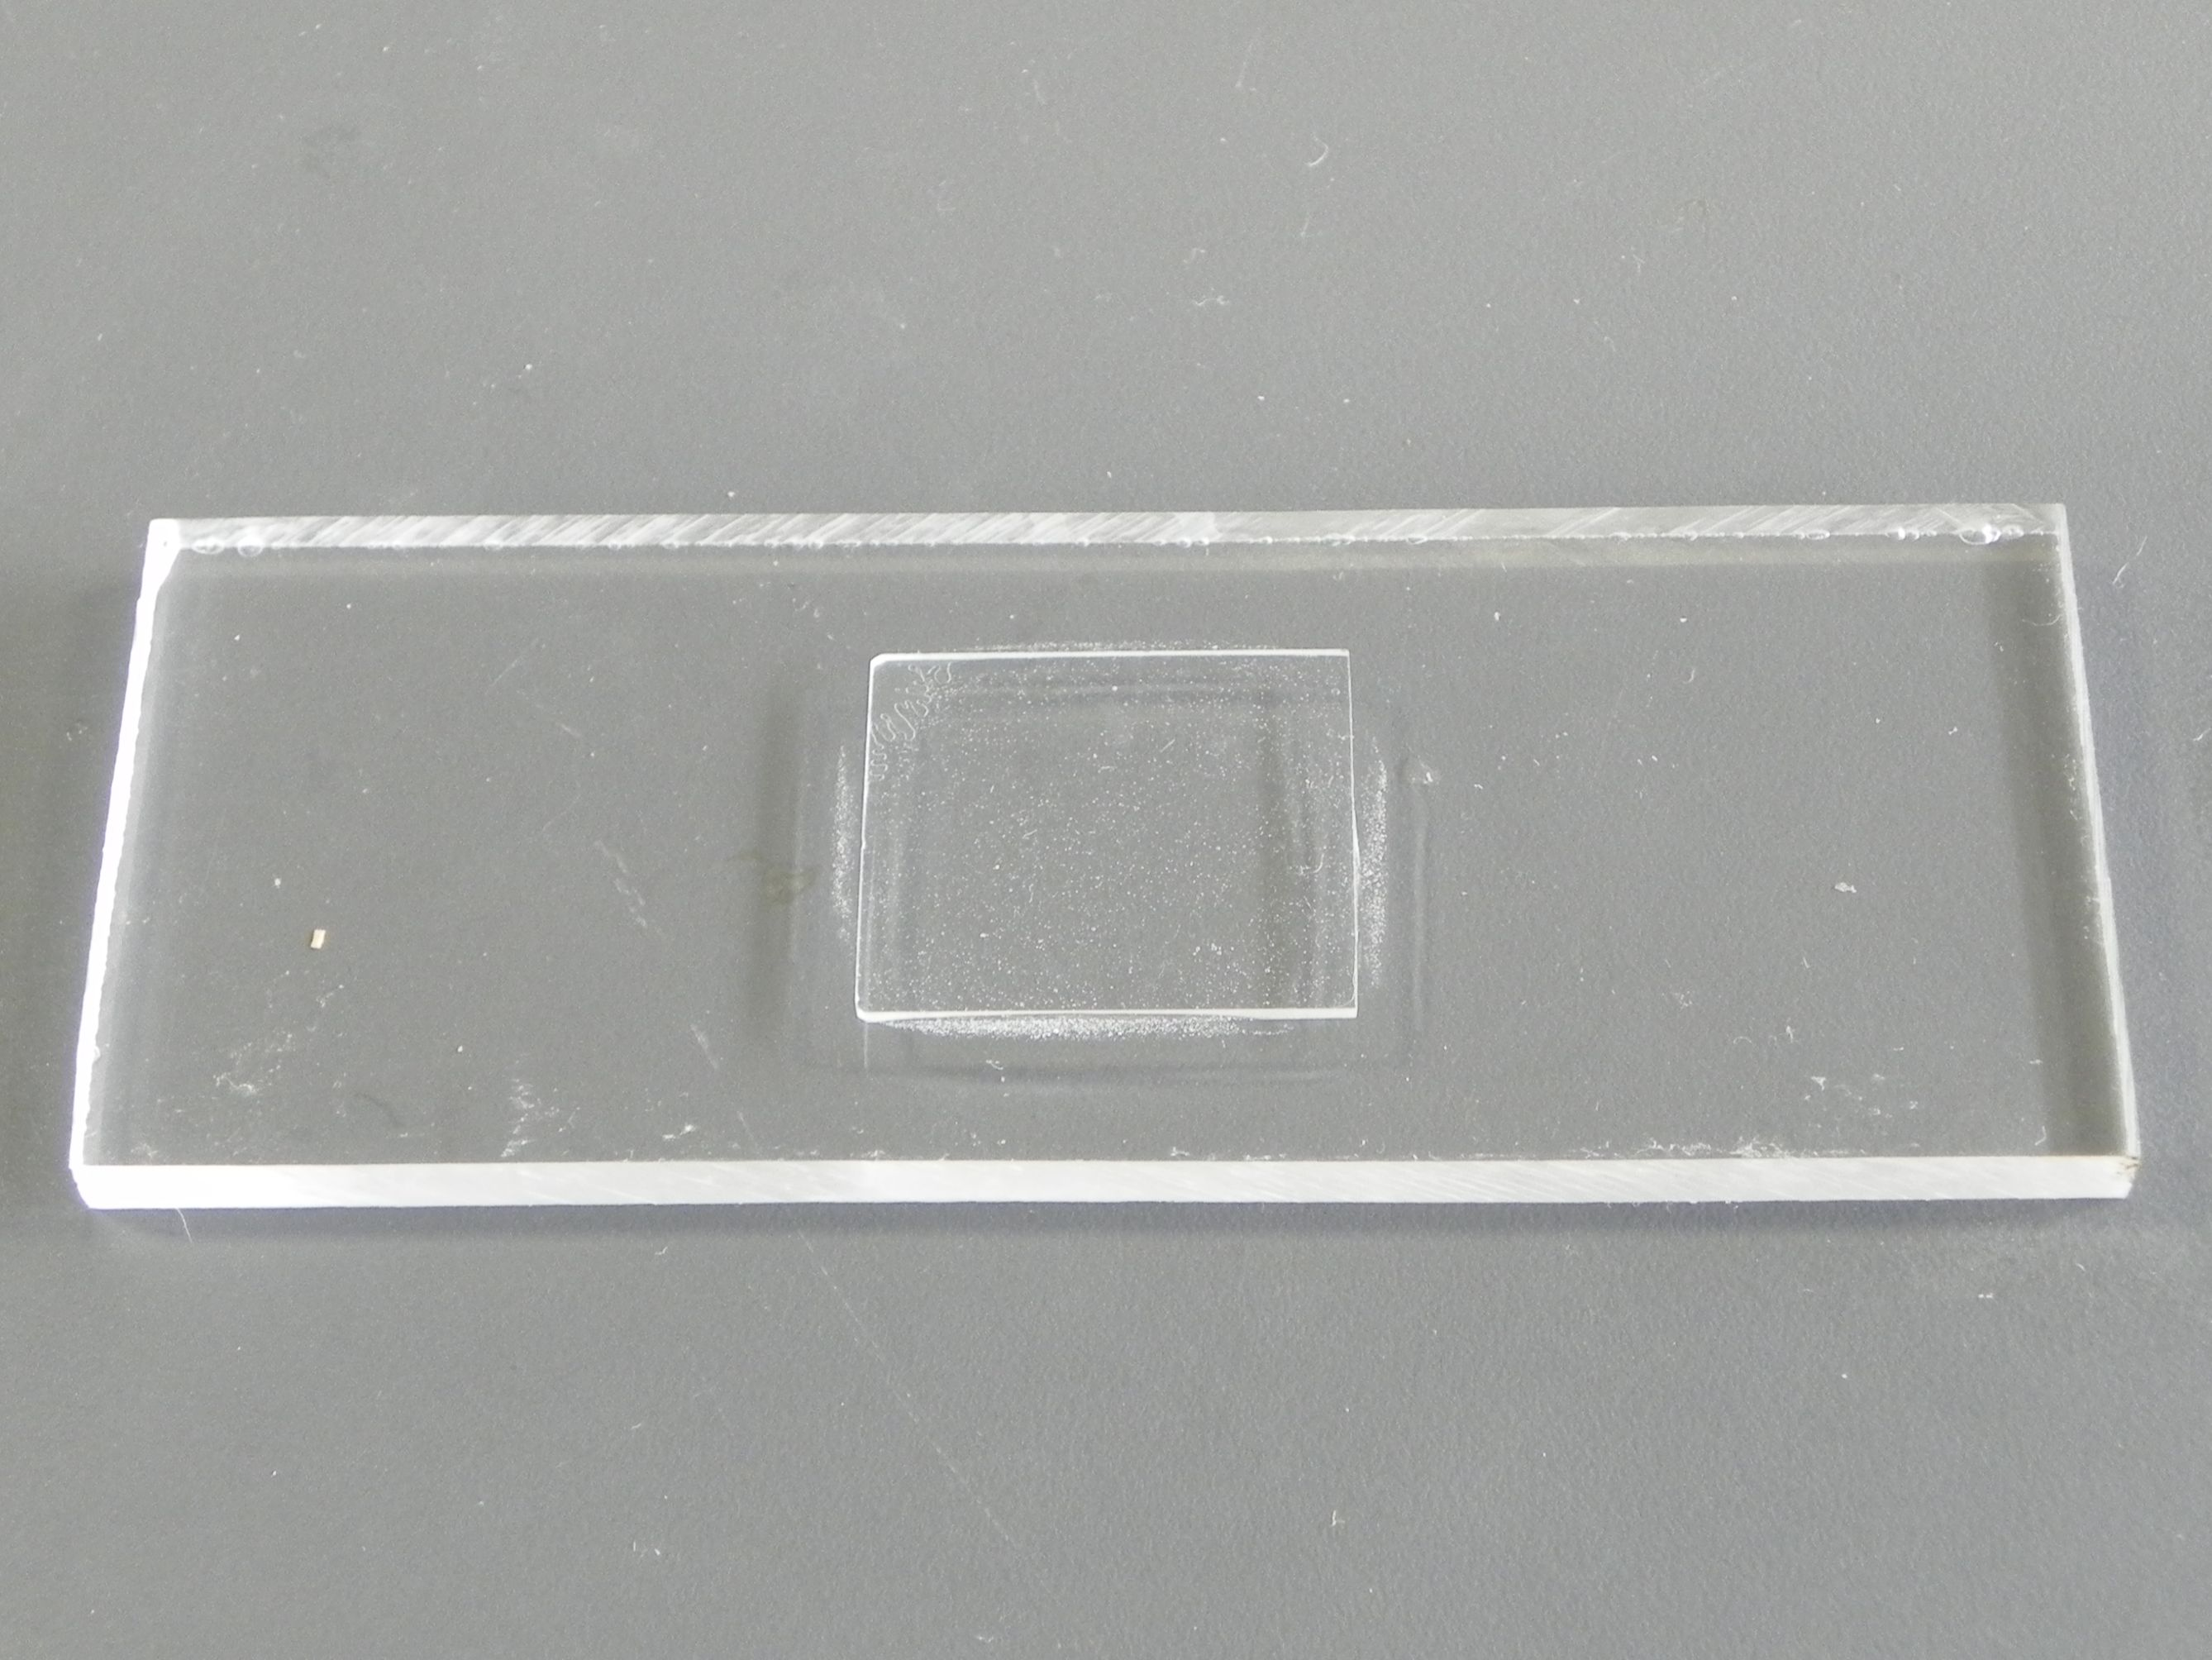
\includegraphics[width=0.5\textwidth]{content/pt1/01-PowerHarvesting/graphics/Photo_streamingPotential_Assembly_Step1.JPG}
      \caption{\label{fig:Photo_streamingPotential_Assembly_Step1}Photo showing half of a glass slide glued to acrylic base plate}
    \end{figure}

    \begin{figure}
      \centering
      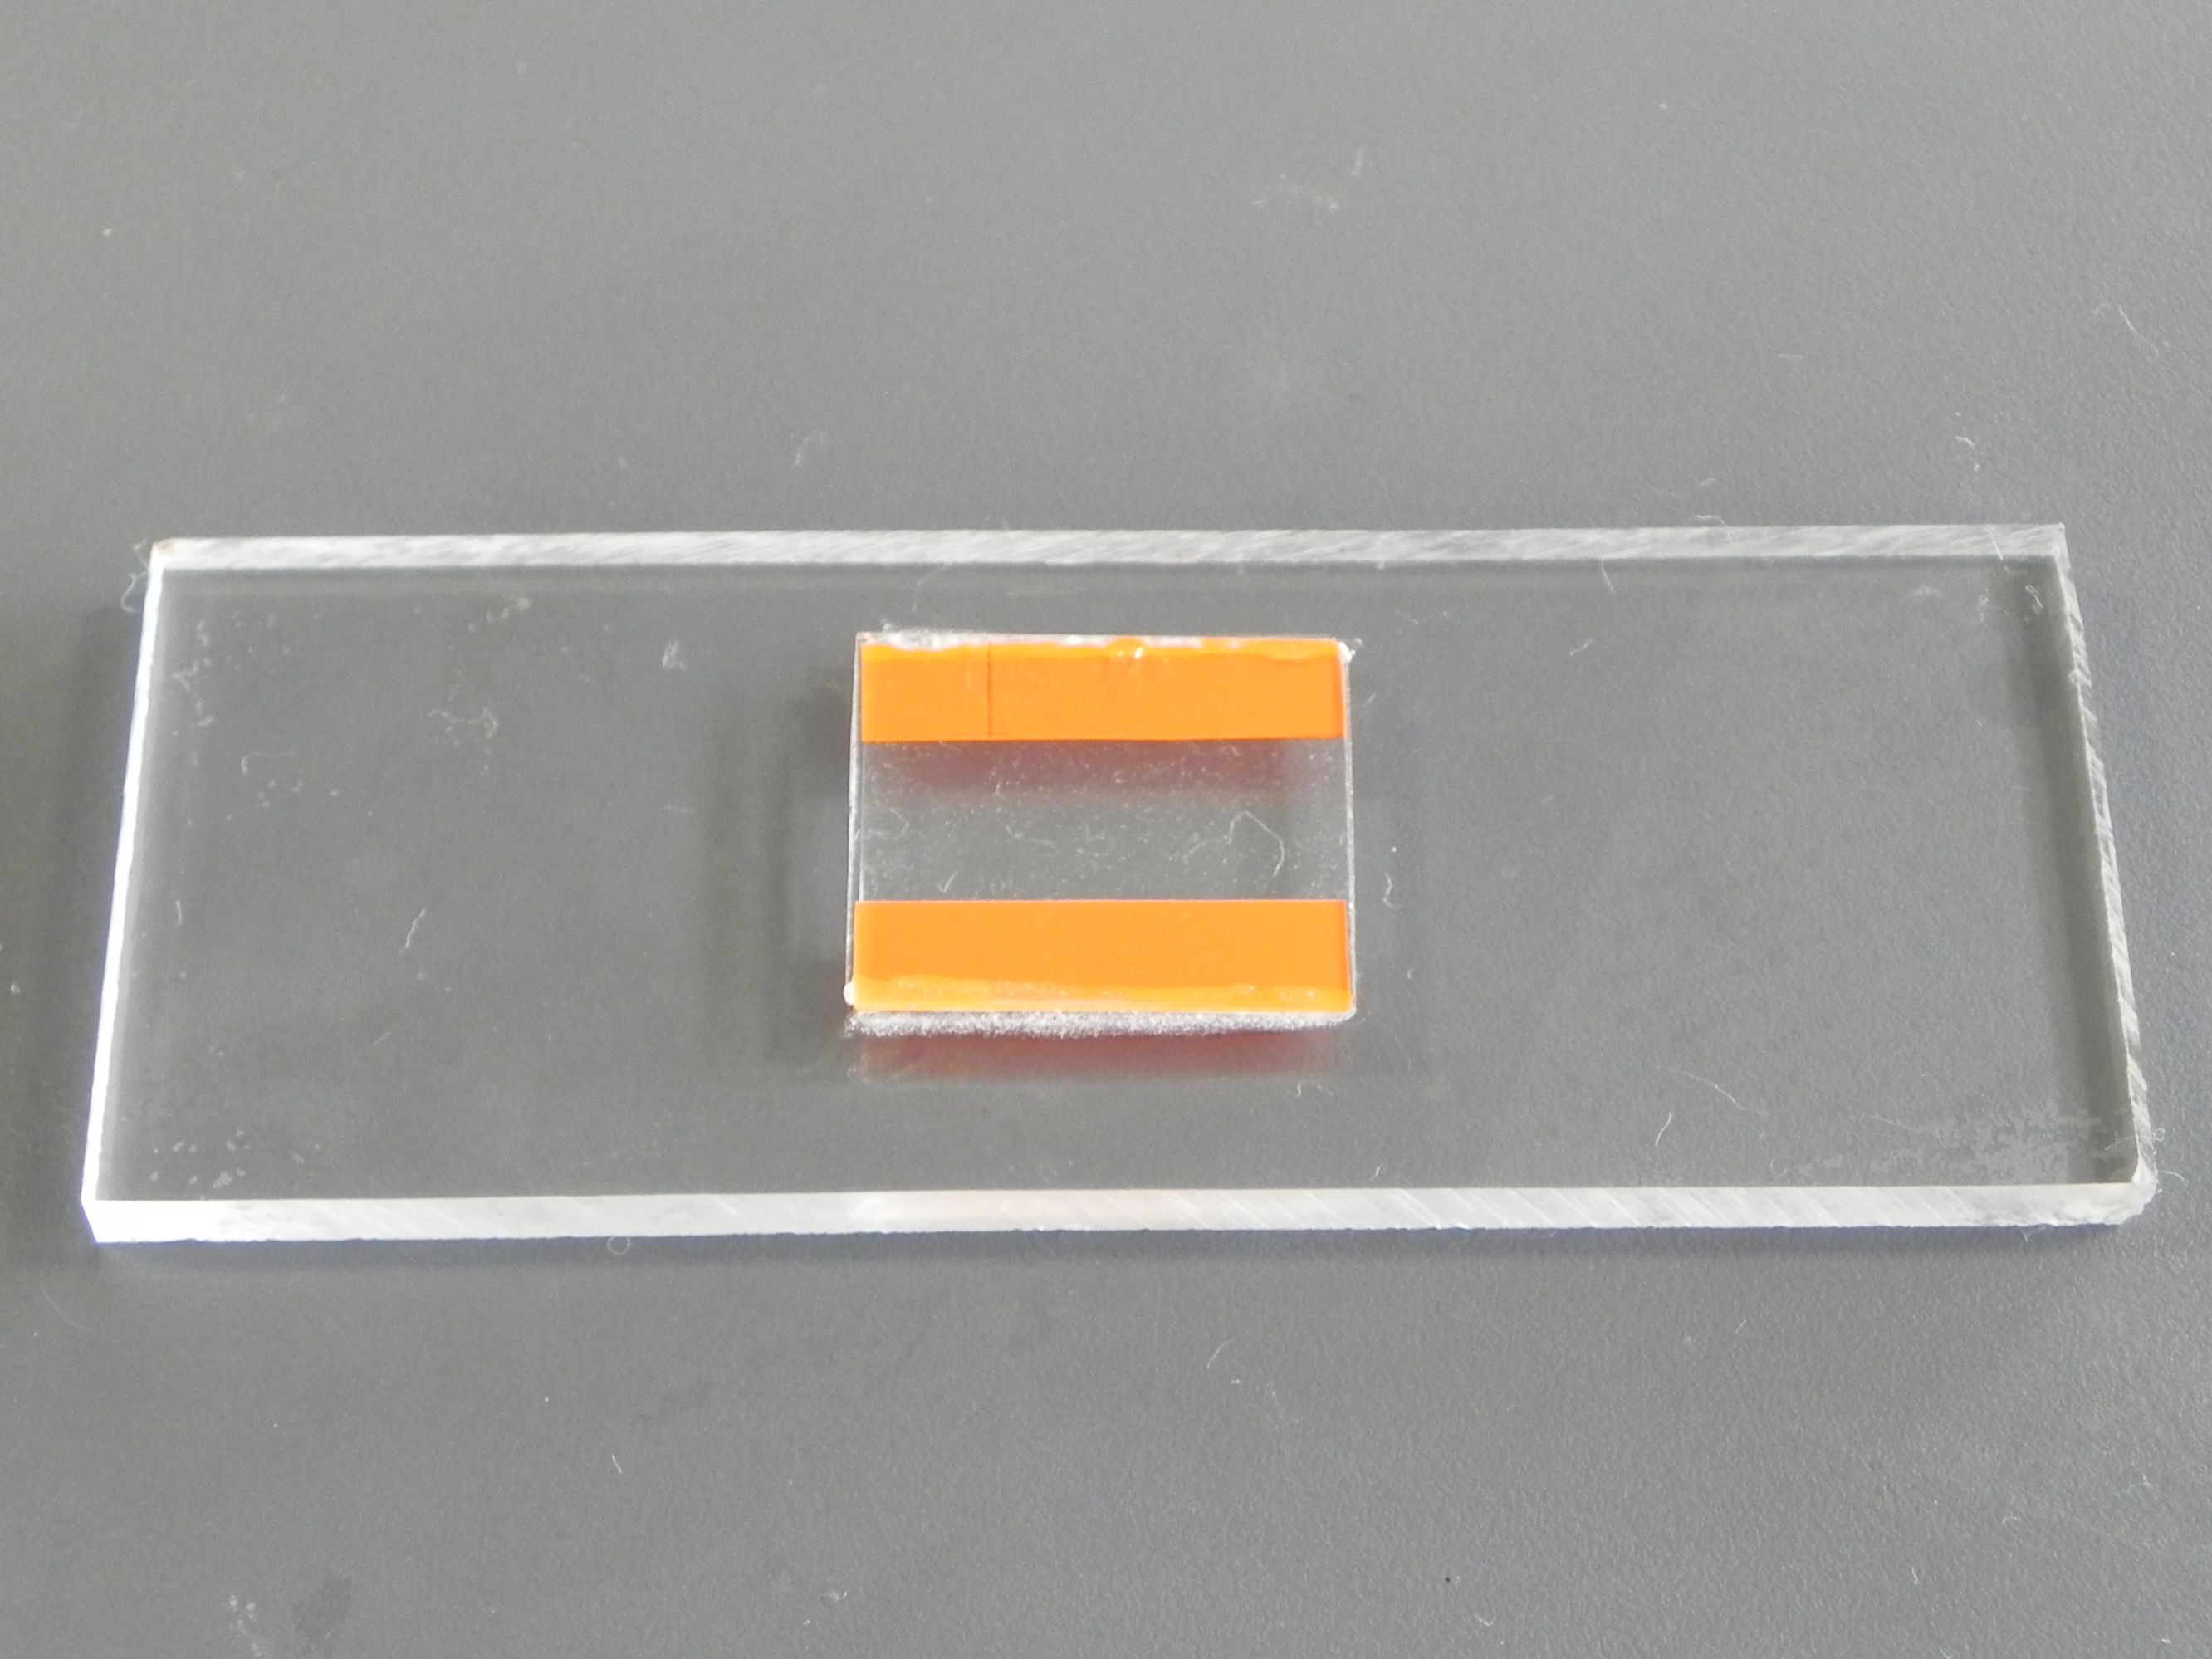
\includegraphics[width=0.5\textwidth]{content/pt1/01-PowerHarvesting/graphics/Photo_streamingPotential_Assembly_Step2.JPG}
      \caption{\label{fig:Photo_streamingPotential_Assembly_Step2}Photo showing plastic shims sandwiched between two slide halves}
    \end{figure}

    \begin{figure}
      \centering
      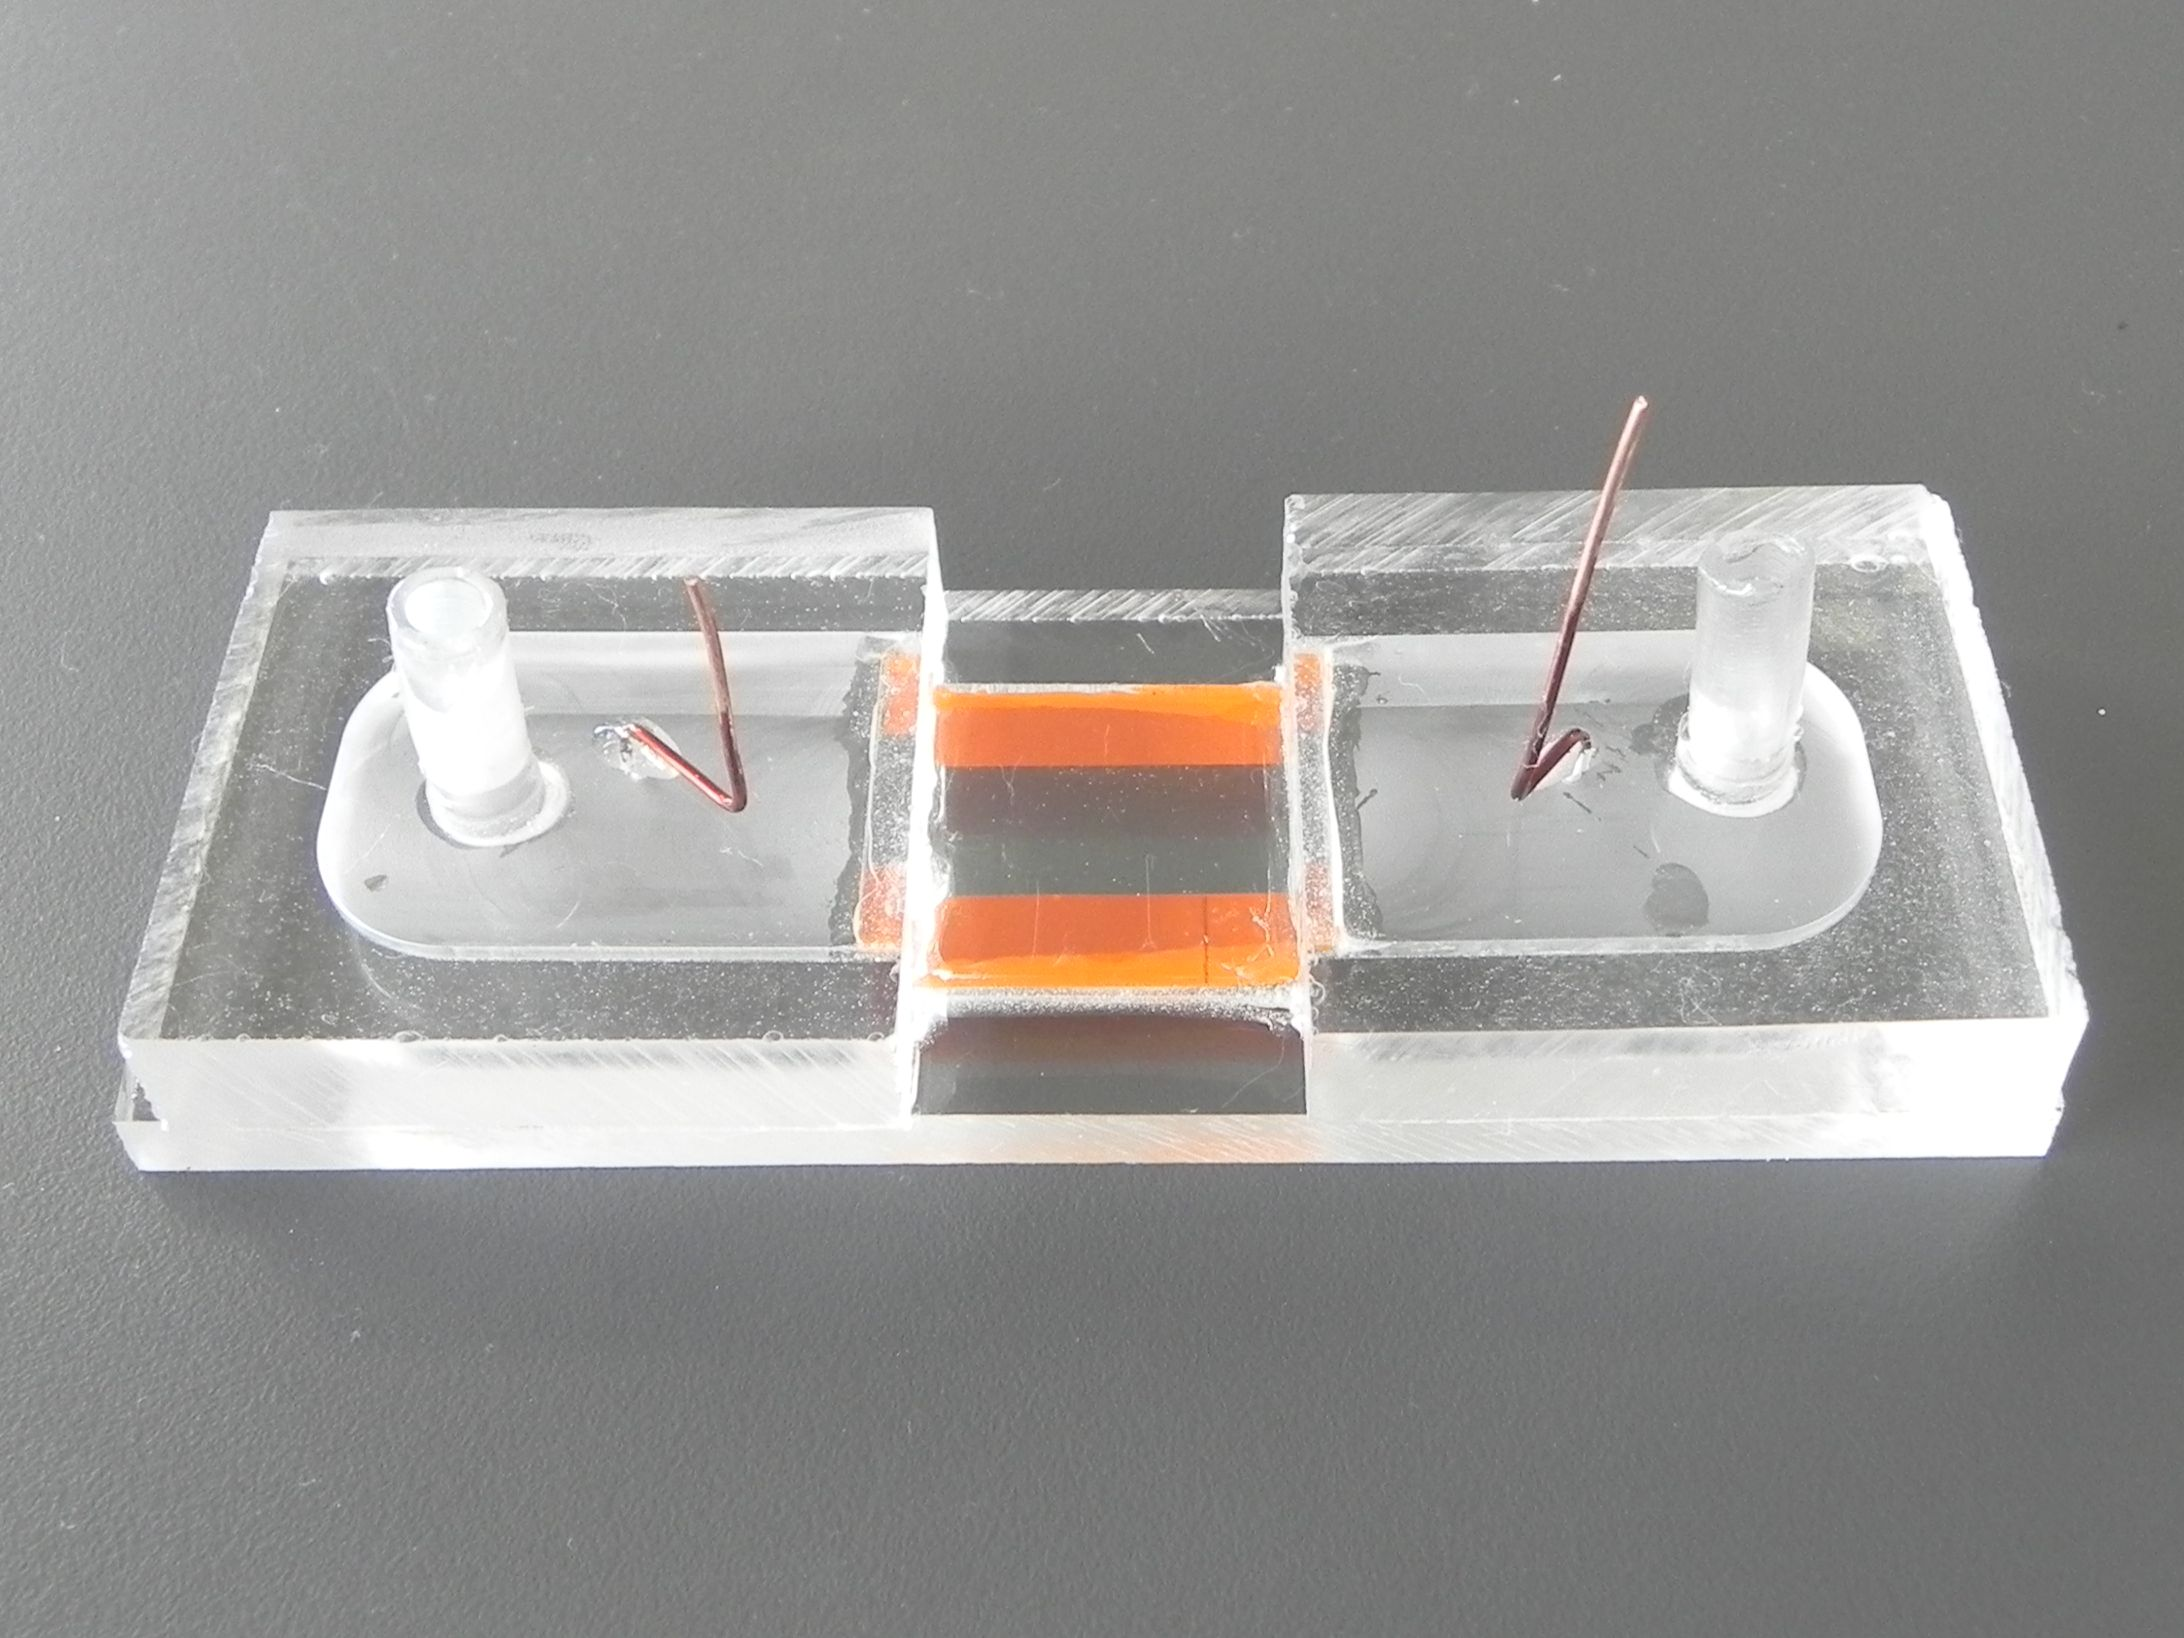
\includegraphics[width=0.5\textwidth]{content/pt1/01-PowerHarvesting/graphics/Photo_streamingPotential_Assembly_Step3.JPG}
      \caption{\label{fig:Photo_streamingPotential_Assembly_Step3}Photo showing final assembly}
    \end{figure}

    \begin{table}
      \begin{tabular}{|c|c|c|} \hline Microscope slides & Sail Brand & JIA 7101WT -
          26 x 76mm\tabularnewline \hline Shims & Garlock & Colorplast - 50$\,\mu$m,
          80$\,\mu$m, 120$\,\mu$m and 250$\,\mu$m\tabularnewline \hline Epoxy &
          Selleys & Araldite - Ultra Clear Resin\tabularnewline \hline Pressure
          Sensor & Honeywell & 24PC15SMT - 0 -- $\pm$15 PSI\tabularnewline \hline
      \end{tabular}
      \caption{\label{Table_StreamingCell_MaterialsUsed}Table of materials used to construct the streaming potential cells}
    \end{table}

    Construction begins by sectioning standard microscope slides into halves.
    This gave glass panels of approximately \SI{26}{\milli\meter} $\times$ \SI{38}{\milli\meter} $\times$ \SI{1}{\milli\meter}.
    Next, a single panel is epoxied to an acrylic base plate.
    A glass panel epoxied to a base plate is shown in Figure~\ref{fig:Photo_streamingPotential_Assembly_Step1}.

    Once set, the plastic shims are cut to the required size, covered with a very thin layer of epoxy, and placed along the edges of the slide.
    The shims line the sides of the glass panel such that they leave a \SI{1}{\centi\meter} gap through the centre.
    A second glass slide is then placed on top of the shims and epoxy resin is used to seal the sides.
    Pressure was applied to the stack while the epoxy set to ensure the epoxy distributed correctly and keep the height narrow.
    A photo of the shims glued between the two slide halves is shown in Figure~\ref{fig:Photo_streamingPotential_Assembly_Step2}.

    Once set, the channel was then examined under a microscope to determine the true internal height of the channel.
    Each of the four corner heights were measured to ensure that the internal channel cavity remained rectangular once fixed in place.

    To finish, acrylic reservoirs where mounted over each end of the channel.
    These reservoirs facilitate the connection of fluid tubes and voltage probes to each end of the channel.
    The final assembly is shown in Figure \ref{fig:Photo_streamingPotential_Assembly_Step3}.
    A full list of materials used to construct the channels is presented as Table~\ref{Table_StreamingCell_MaterialsUsed}.

    A total of 10 channels were made and tested using this method.

  \subsubsection*{Experimental setup}

    Measurement of the harvester's output was made in a laboratory with high-sensitivity measurement apparatus and a lab tap for the application water pressure.

    Output power was measured using precision source measurement units (SMU).
    Applied pressure was measured using a differential pressure sensor.

    The Agilent E5270B is a mainframe system that holds banks of SMUs with connections to a GPIB computer interface.
    The Department of Engineering's E5270 contains three SMUs, each having the ability to measure currents as low as one femto-ampere.
    The device uses force and sense lines to ensure the voltage/current being set is accurately controlled at the desired point within the test device.
    Additionally, it uses tri-axial cables to minimise any interference from outside sources.

    The input impedance to the E5270's measurement units are specified as \SI{13}{\giga\ohm}.
    It is essential to use such a high impedance measurement due to the high internal resistance of the cell.
    I later show that the internal electrical resistance of the cell is in the order of \SI{5}{\mega\ohm}.
    If using a lab multimeter, typical internal resistance of \SI{10}{\mega\ohm}, its internal resistance is too close to that of the cells and will affect the measured output.

    The type of differential pressure sensor used was a Honeywell 26PC SMT Series sensor.
    It comes with a surface mount package but was a cost effective solution, adequate for our requirements.
    Internally it contains a bridge circuit as shown in figure \ref{fig:PressureSensorSchematic}.
    \begin{figure}
        \centering
        
\includegraphics{content/pt1/01-PowerHarvesting/graphics/PressureSensorSchematic}
        \caption{\label{fig:PressureSensorSchematic}Circuit diagram of the differential pressure sensor bridge circuit (taken from \cite{Honeywell2003})}
    \end{figure}
    It has two narrow ports to which rubber tubes are attached and pressure is applied.
    By applying \SI{10}{\volt} DC to across the devices power pins, the voltage difference across outputs A and B is corresponds to the applied pressure difference.
    This output voltage difference was measured using the precision measurement mainframe, but was powered using an Agilent E3631A bench-top power supply.

    The mainframe was controlled from a PC running Python scripts utilising the open source Python-vxi11 library~\cite{Python-ivi2014}.
    This allows sweeping the amount of current drawn from the harvester while recording the corresponding voltage drop.
    This is the equivalent of varying the load resistance across the harvester, which allows us to find the point of maximum power transfer.

    A diagram showing the measurement setup is shown in figure~\ref{fig:measurementSetup}.
    It shows connection of the measurement mainframe, benchtop power supply, streaming cell, pressure sensor, and the lab tap.
    Table~\ref{tab:measurementSetup_legend} provides details of the abbreviated electrical connection labels used in the figure~\ref{fig:measurementSetup}.

    \begin{figure}
        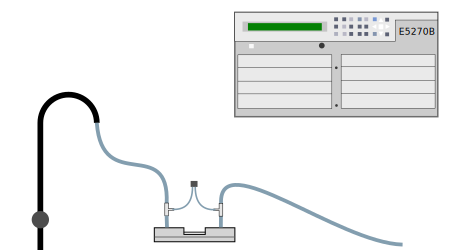
\includegraphics{content/pt1/01-PowerHarvesting/graphics/measurementSetup}
        \caption{\label{fig:measurementSetup}Diagram of equipment setup while measuring power output from the streaming cell harvesters}
    \end{figure}

    \begin{table}
        \centering
        \begin{tabular}{r|l}
        CELL - A & Voltage/current at high-pressure side of cell\\
        PRESS. - A & Output A of pressure sensor\\
        PRESS. - B & Output B of pressure sensor\\
        CELL - B & Voltage/current at low-pressure side of cell
        \end{tabular}
        \caption{\label{tab:measurementSetup_legend}Description of labels used in streaming cell measurement setup diagram}
    \end{table}

    \subsubsection*{Measurement issues}

    There are two issues with the measurement setup that may impact the measurements.
    Firstly, the electrodes used were copper and are susceptible to electrolysis.
    Secondly, the differential pressure sensor is only rated to 15\thinspace PSI (approximately \SI{100}{\kilo\pascal}), less than half the maximum pressure developed across the cell.

    Electrolysis on at the electrode surface causes the electrodes to polarise, resulting in a measurable voltage offset across the electrodes without applied pressure.
    The voltage is opposite in polarity to the voltage developed while the electrodes are in operation.
    By reversing the flow of water through the cell, the polarisation can be reversed.
    Use of more suitable electrode materials would reduce this effect, for instance platinum black electrodes.
    Copper was used for the electrodes as it was cheap, easily obtainable and easy to work with.

    From measurement of the output voltage of the cells, the presented graphs and figures have been adjusted to remove the effects of electrolysis.
    This shifts the y-intercept up to \SI{0}{\volt} where no pressure is applied to the cell.
    I believe this provides a more accurate representation of the situation had platinum black electrodes been used.
    As no absolute data is taken from these measurements, the y-intercept adjustment does not affect any subsiquent predictions made about the cells.
    Only the gradient of the output, relative to the pressure applied is used; and even then, only to select a suitable candidate cell for power measurement.
    \emph{Most importantly}, no offsets have been applied to measurements of the cell power output.

    Although the maximum rated pressure of sensor was 15\thinspace PSI (approximately \SI{100}{\kilo\pascal}), the sensor's output remained linear up to our maximum pressure of 40\thinspace PSI (\SI{275}{\kilo\pascal}).
    I expect that exceeding the sensors specified pressure will result in a lower `mean time to failure', but its output remained true.
    As a precaution, a tyre pressure gauge was used to roughly confirm the output of the sensor at the end of the cell measurements.
    This was a crude test, however it's output matched that of the differential pressure sensor, so was a good indication of its repeatability.


\subsection{Results}

Results from streaming cell measurement are broken into two sub-sections.
The first sub-section presents the output voltage of the ten cells in response to applied water pressure.
From these measurements, the cell with the highest voltage/pressure ratio is found.
The second sub-section shows the maximum power that can be harvested from that cell.
These are the most important measurements as they reveal the energy conversion efficiency of the cells.

\subsubsection*{Voltage versus pressure:}


\begin{figure}[p]
    \centering
    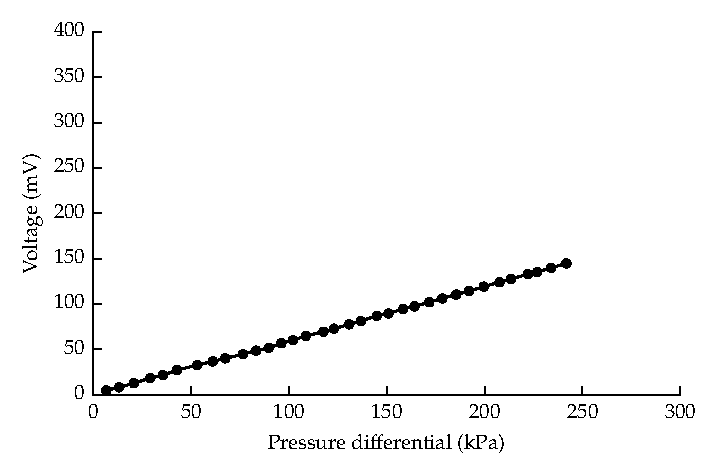
\includegraphics{content/pt1/01-PowerHarvesting/graphics/streamingCell_voltVsPress_26um_out}
    \caption{\label{fig:VvsP_26um}Graph showing the voltage output with applied pressure differential across a \SI{26}{\micro\metre} glass micro-channel (\SI{38}{\milli\volt} offset added)}
\end{figure}

\begin{figure}
    \centering
    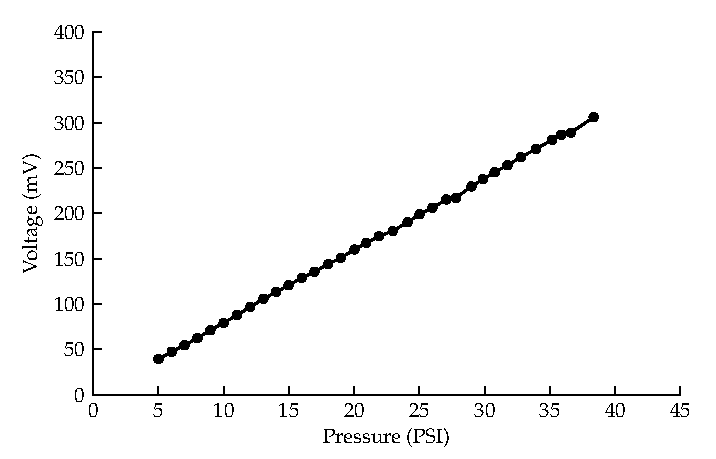
\includegraphics{content/pt1/01-PowerHarvesting/graphics/streamingCell_voltVsPress_52um_out}
    \caption{\label{fig:VvsP_52um}Graph showing the voltage output with applied pressure differential across a \SI{52}{\micro\metre} glass micro-channel (\SI{23}{\milli\volt} offset added)}
\end{figure}

\begin{figure}
    \centering
    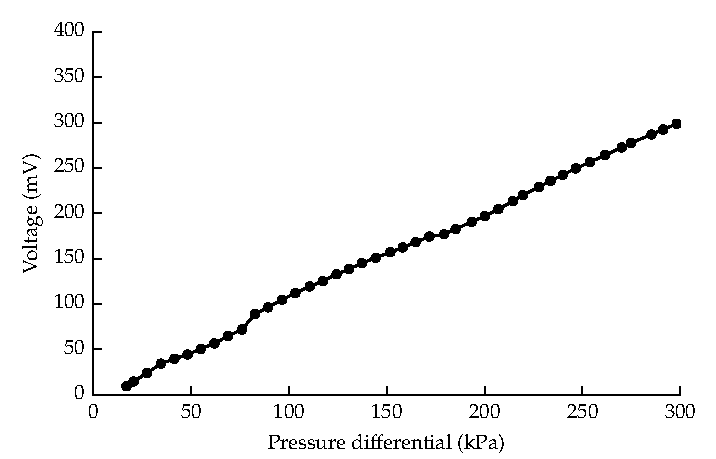
\includegraphics{content/pt1/01-PowerHarvesting/graphics/streamingCell_voltVsPress_56um_out}
    \caption{\label{fig:VvsP_56um}Graph showing the voltage output with applied pressure differential across a \SI{56}{\micro\metre} glass micro-channel (\SI{405}{\milli\volt} offset added)}
\end{figure}

\begin{figure}
    \centering
    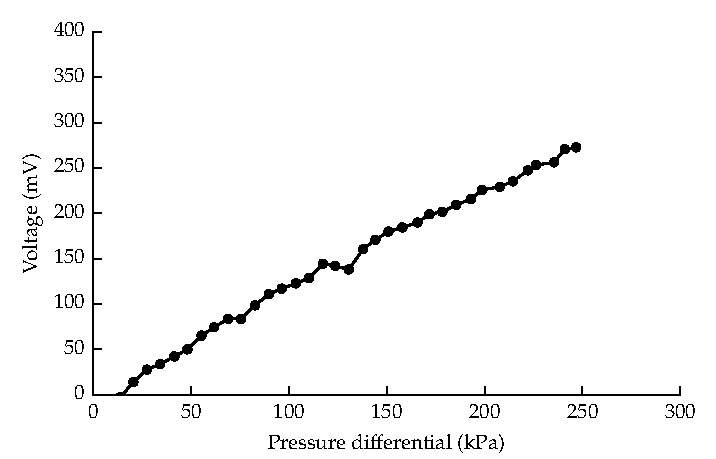
\includegraphics{content/pt1/01-PowerHarvesting/graphics/streamingCell_voltVsPress_71um_out}
    \caption{\label{fig:VvsP_71um}Graph showing the voltage output with applied pressure differential across a \SI{71}{\micro\metre} glass micro-channel (\SI{44}{\milli\volt} offset added)}
\end{figure}

\begin{figure}
    \centering
    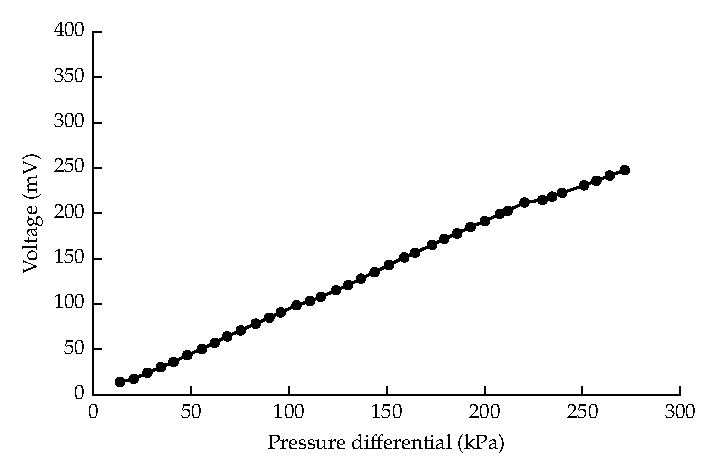
\includegraphics{content/pt1/01-PowerHarvesting/graphics/streamingCell_voltVsPress_75um_out}
    \caption{\label{fig:VvsP_75um}Graph showing the voltage output with applied pressure differential across a \SI{75}{\micro\metre} glass micro-channel (\SI{20}{\milli\volt} offset added)}
\end{figure}

\begin{figure}
    \centering
    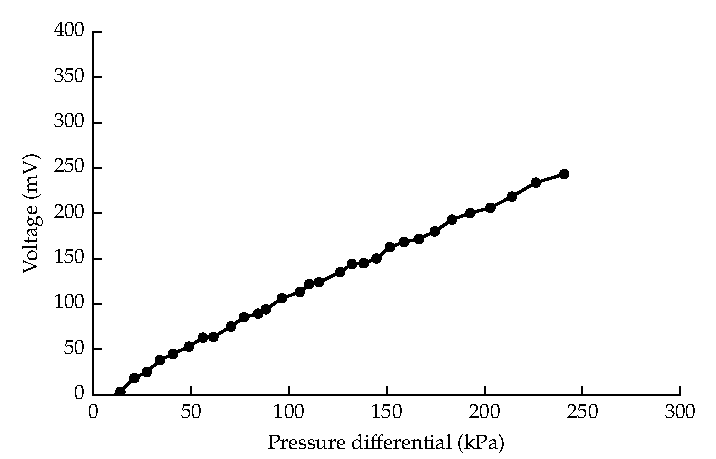
\includegraphics{content/pt1/01-PowerHarvesting/graphics/streamingCell_voltVsPress_106um_out}
    \caption{\label{fig:VvsP_106um}Graph showing the voltage output with applied pressure differential across a \SI{106}{\micro\metre} glass micro-channel (\SI{56}{\milli\volt} offset added)}
\end{figure}

\begin{figure}
    \centering
    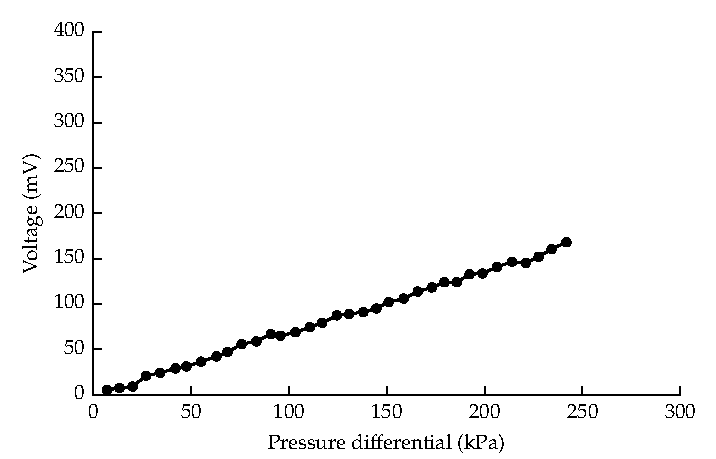
\includegraphics{content/pt1/01-PowerHarvesting/graphics/streamingCell_voltVsPress_125um_out}
    \caption{\label{fig:VvsP_125um}Graph showing the voltage output with applied pressure differential across a \SI{125}{\micro\metre} glass micro-channel (\SI{5}{\milli\volt} offset added)}
\end{figure}

\begin{figure}
    \centering
    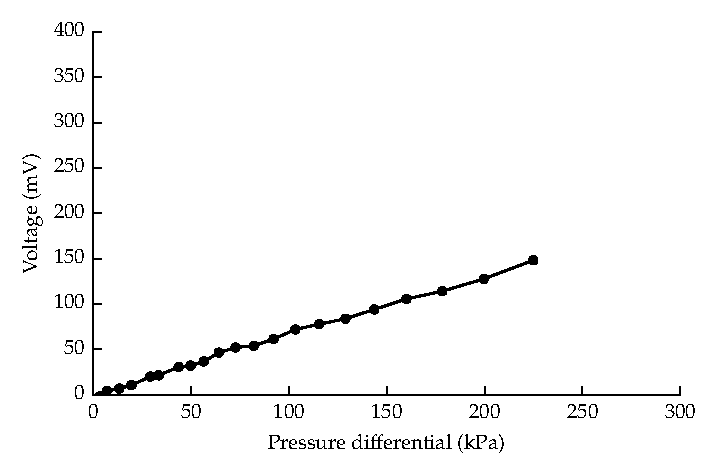
\includegraphics{content/pt1/01-PowerHarvesting/graphics/streamingCell_voltVsPress_161um_out}
    \caption{\label{fig:VvsP_161um}Graph showing the voltage output with applied pressure differential across a \SI{161}{\micro\metre} glass micro-channel (\SI{23}{\milli\volt} offset added)}
\end{figure}

\begin{figure}
    \centering
    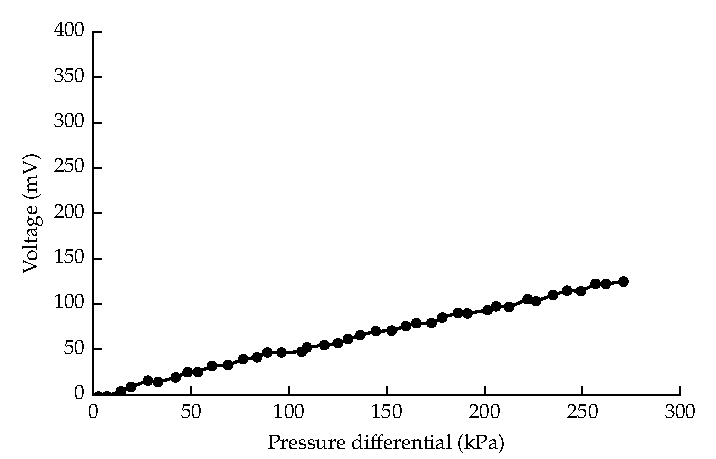
\includegraphics{content/pt1/01-PowerHarvesting/graphics/streamingCell_voltVsPress_178um_out}
    \caption{\label{fig:VvsP_178um}Graph showing the voltage output with applied pressure differential across a \SI{178}{\micro\metre} glass micro-channel (\SI{13}{\milli\volt} offset added)}
\end{figure}

\begin{figure}
    \centering
    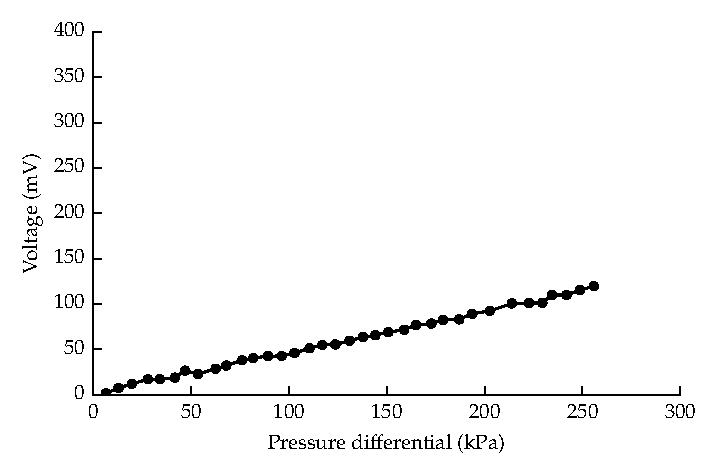
\includegraphics{content/pt1/01-PowerHarvesting/graphics/streamingCell_voltVsPress_245um_out}
    \caption{\label{fig:VvsP_245um}Graph showing the voltage output with applied pressure differential across a \SI{245}{\micro\metre} glass micro-channel (\SI{27}{\milli\volt} offset added)}
\end{figure}

\Crefrange{fig:VvsP_26um}{fig:VvsP_245um} show the results of voltage only measurements from each of the ten cells.
They represent the first successful measurements I had made of streaming cells.
During these measurements, three cells burst under pressure, two were dropped and subsequently shattered and one suffered epoxy failure, loosing the acrylic base plate.

No measurements of flow rate or output current were made during these early experiments.
As a result they reveal very little about the efficiency of the cells themselves.
We cannot determine either the mechanical energy put into the cells, nor the output power available.

\Cref{fig:VvsP_56um,fig:VvsP_71um} gave poor measurements.
\Cref{fig:VvsP_56um} required an offset adjustment of \SI{405}{\milli\volt} before its slope gave a \SI{0}{\milli\volt} intercept.
This places its output well out of range the chart before any pressure was applied; clearly highly polarised by the time these measurements were made.
\Cref{fig:VvsP_71um} shows some instability at the output, most probably as a result of inconsistent flow through the cell.
The remaining figures show the linearity of the cell output.

\begin{figure}
    \centering
    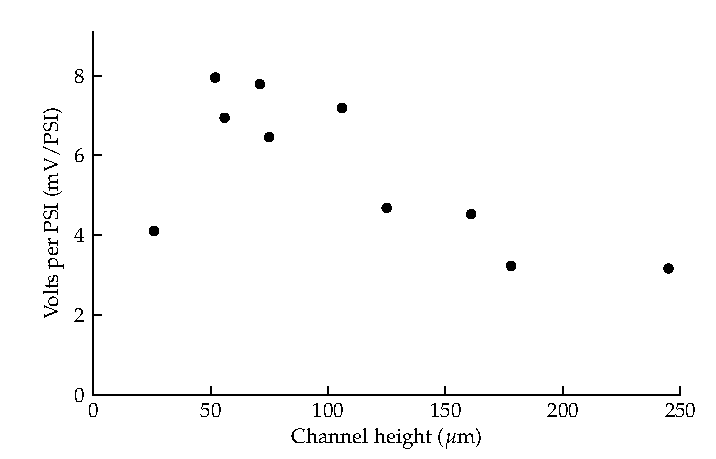
\includegraphics{content/pt1/01-PowerHarvesting/graphics/streamingCell_slopeVsChannelHeight}
    \caption{\label{fig:streamingCell_scatter_voltGradVsHeight}Scatter plot of voltage/pressure gradient versus channel height for each of the measured channels.}
\end{figure}

\Cref{fig:streamingCell_scatter_voltGradVsHeight} collects the output slopes form each of the previous graphs and plots them against the internal channel height for each cell.

Because the output of each of the cells were measured using a suitably large impedance voltage measurement (in the order of \SI{13}{\giga\ohm}), we assume that insufficient current is drawn by the measurement to affect the output voltage.



\subsubsection*{Power versus output resistance}


% The first shows voltage measurements of the ten cells, adjusted to remove the effects of electrolysis.
% From these measurements, the

% Ten cavities ranging in height from 26$\,\mu m$ to 245$\,\mu m$ where built and
% measured. Individual plots showing pressure applied versus voltage developed
% are shown in Appendix \ref{sec:Appendix-Streaming-Potential-Cell}.  For
% convenience, a graph with the steepest voltage per pressure gradient is shown
% in Figure \ref{fig:streamingCell_voltVsPress_52um_convienient}, which resulted
% from using a cell with a height of 52$\,\mu m$.



% From the results obtained it is clear that there is a definite \nobreakdash-
% linear \nobreakdash- relationship between the amount of pressure applied and
% the voltage developed across each channel. Figure
% \ref{fig:streamingCell_scatter_voltGradVsHeight} compares the gradient of
% voltage developed per PSI of pressure for each of the channels. The graph shows
% a trend toward larger voltage development as channel height is reduced to
% around 50$\,\mu m$. Below 50$\,\mu m$ it is unclear what to expect from the
% channel which will require further investigation. Spread in the data is
% expected to be the result of epoxy (used to glue the slides together) seeping
% into the cavity, thereby slightly altering each cavity's dimensions.




\subsection{Conclusion}

Power generation from streaming potential cells is possible, this is evident
from the voltages developed in this experiment. The streaming cell is capable
of producing output when operated using standard tap water at standard tap
pressures. As yet, the amount of current that can be drawn from such a channel
has not been ascertained, and therefore the amount of available power remains
unknown (although it is estimated to be in the very small). An initial estimate
of the ideal channel lies between 25-75$\,\mu m$ in height.

